\documentclass[border=5pt, multi, tikz]{standalone}
\usetikzlibrary{quotes,arrows.meta}

\definecolor{red}{rgb}{1,.5,.6}
\definecolor{blue}{rgb}{.5,.5,1}
\definecolor{purple}{rgb}{.75,.5,.8}

\begin{document}
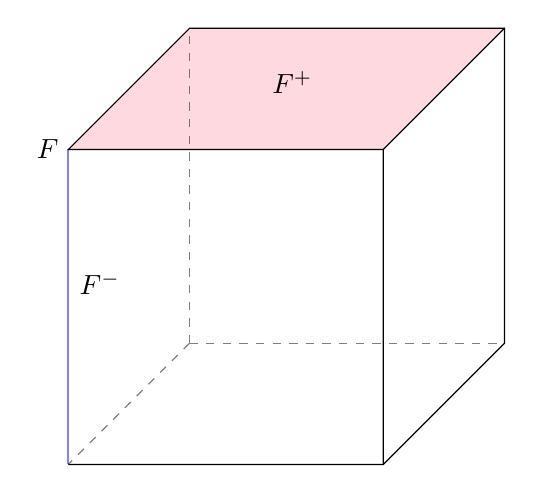
\begin{tikzpicture}
\coordinate (o) at (0,0,0);
\coordinate (a) at (-4,0,0);
\coordinate (b) at (-4,-4,0);
\coordinate (c) at (0,-4,0);
\coordinate (d) at (0,-4,-4);
\coordinate (e) at (0,0,-4);
\coordinate (f) at (-4,0,-4);
\coordinate (g) at (-4,-4,-4);

\draw[fill, color=red, opacity=.3] (o) -- (a) -- (f) -- (e);
\draw[blue, thick] (a)--(b);
\path[dashed, opacity=.5] (g) edge (b) edge (d) edge (f);
\draw (o) -- (a) -- (f) -- (e) -- (d) -- (c) -- (b);
\draw (c) -- (o) -- (e);

\node at (-3.6, -1.7, 0) {$F^-$};
\node[left] at (a) {$F$};
\node at (0, 2, 3) {$F^+$};

%\node at (o){o};
%\node at (a){a};
%\node at (b){b};
%\node at (c){c};
%\node at (d){d};
%\node at (e){e};
%\node at (f){f};
%\node at (g){g};
\end{tikzpicture}
\end{document}

















